\documentclass[a4paper,11pt]{report}
\usepackage{chuan_math_gkt}
\usetikzlibrary{angles,quotes,intersections,patterns,decorations.pathreplacing}
\chuanexamsetup

\begin{document}
\examfontsize

\examsecret{绝密$\bigstar$启用前}

\examtitle{2023年普通高等学校招生全国统一考试（全国乙卷文科）}{数\quad 学}

\noticetitle
\begin{examnotice}
\item 答卷前，考生务必将自己的姓名、准考证号填写在答题卡上. 
\item 回答选择题时，选出每小题的答案后，用铅笔把答题卡上对应题目的答案标号涂黑. 如需改动，用橡皮擦干净后，再选涂其他答案标号. 回答非选择题时，将答案写在答题卡上. 写在本试卷上无效. 
\item 考试结束后，将本试卷和答题卡一并交回. 
\end{examnotice}

\examsection{一、选择题：本题共12小题，每小题5分，共60分. 在每小题给出的四个选项中，只有一项是符合题目要求的. }
\begin{examquestions}
\item $|2+\mathrm{i}^2+2\mathrm{i}^3|=$
\fourchoices{$1$}{$2$}{$\sqrt5$}{$5$}
\item 设全集$U=\{0,1,2,4,6,8\}$，集合$M=\{0,4,6\}$，$N=\{0,1,6\}$，则$M\cup\complement_U N=$
\fourchoices{$\{0,2,4,6,8\}$}{$\{0,1,4,6,8\}$}{$\{1,2,4,6,8\}$}{$U$}
\item 如图，网格纸上绘制的一个零件的三视图，网格小正方形的边长为$1$，则该零件的表面积为
\begin{tightcenter}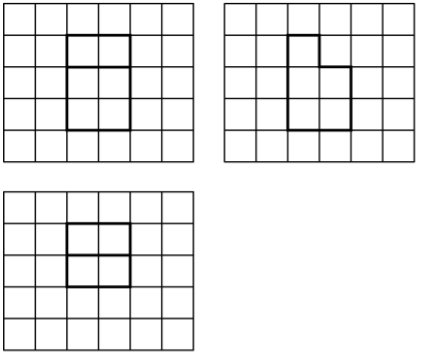
\includegraphics[width=3.6cm]{figures/2023_yi_li_q3.png}\end{tightcenter}
\fourchoices{$24$}{$26$}{$28$}{$30$}
\item 在$\triangle ABC$中，内角$A,B,C$的对边分别是$a,b,c$，若$a\cos B-b\cos A=c$，且$C=\dfrac\pi5$，则$\angle B=$
\fourchoices{\tallchoice{$\dfrac\pi{10}$}}{\tallchoice{$\dfrac\pi5$}}{\tallchoice{$\dfrac{3\pi}{10}$}}{\tallchoice{$\dfrac{2\pi}5$}}
\item 已知$f(x)=\dfrac{xe^x}{e^{ax}-1}$是偶函数，则$a=$
\fourchoices{$-2$}{$-1$}{$1$}{$2$}
\item 正方形$ABCD$的边长是$2$，$E$是$AB$的中点，则$\vec{EC}\cdot\vec{ED}=$
\fourchoices{$\sqrt5$}{$3$}{$2\sqrt5$}{$5$}
\item 设$O$为平面坐标系的坐标原点，在区域$\{(x,y)\mid 1\leq x^2+y^2\leq4\}$内随机取一点$A$，则直线$OA$的倾斜角不大于$\dfrac\pi4$的概率为
\fourchoices{\tallchoice{$\dfrac18$}}{\tallchoice{$\dfrac16$}}{\tallchoice{$\dfrac14$}}{\tallchoice{$\dfrac12$}}
\item 函数$f(x)=x^3+ax+2$存在$3$个零点，则$a$的取值范围是
\fourchoices{$(-\infty,-2)$}{$(-\infty,-3)$}{$(-4,-1)$}{$(-3,0)$}
\item 某学校举办作文比赛，共$6$个主题，每位参赛同学从中随机抽取一个主题准备作文，则甲、乙两位参赛同学抽到不同主题概率为
\fourchoices{\tallchoice{$\dfrac56$}}{\tallchoice{$\dfrac23$}}{\tallchoice{$\dfrac12$}}{\tallchoice{$\dfrac13$}}
\item 已知函数$f(x)=\sin(\omega x+\varphi)$在区间$\left(\dfrac\pi6,\dfrac{2\pi}3\right)$单调递增，直线$x=\dfrac\pi6$和$x=\dfrac{2\pi}3$为函数$y=f(x)$的图像的两条对称轴，则$f\left(-\dfrac{5\pi}{12}\right)=$
\fourchoices{\tallchoice{$-\dfrac{\sqrt3}{2}$}}{\tallchoice{$-\dfrac12$}}{\tallchoice{$\dfrac12$}}{\tallchoice{$\dfrac{\sqrt3}{2}$}}
\item 已知实数$x,y$满足$x^2+y^2-4x-2y-4=0$，则$x-y$的最大值是
\fourchoices{\tallchoice{$1+\dfrac{3\sqrt2}{2}$}}{$4$}{$1+3\sqrt2$}{$7$}
\item 设$A,B$为双曲线$x^2-\dfrac{y^2}{9}=1$上两点，下列四个点中，可为线段$AB$中点的是
\fourchoices{$(1,1)$}{$(-1,2)$}{$(1,3)$}{$(-1,-4)$}
\end{examquestions}

\examsection{二、填空题：本题共4小题，每小题5分，共20分. }
\begin{examquestions}[start=13]
\item 已知点$A(1,\sqrt5)$在抛物线$C:y^2=2px$上，则$A$到$C$的准线的距离为\blank. 
\item 若$\theta\in\left(0,\dfrac\pi2\right)$，$\tan\theta=\dfrac12$，则$\sin\theta-\cos\theta=$\blank. 
\item 若$x,y$满足约束条件\linsys{x-3y\leq -1,\\x+2y\leq9,\\3x+y\geq7}，则$z=2x-y$的最大值为\blank. 
\item 已知点$S,A,B,C$均在半径为$2$的球面上，$\triangle ABC$是边长为$3$的等边三角形，$SA\perp$平面$ABC$，则$SA=$\blank. 
\end{examquestions}
\newpage
\examsection{三、解答题：本题共6小题，共70分. 解答应写出文字说明、证明过程或演算步骤. }
\begin{examanswers}[start=17]
\item（12分）

某厂为比较甲乙两种工艺对橡胶产品伸缩率的处理效应，进行$10$次配对试验，每次配对试验选用材质相同的两个橡胶产品，随机地选其中一个用甲工艺处理，另一个用乙工艺处理，测量处理后的橡胶产品的伸缩率. 甲、乙两种工艺处理后的橡胶产品的伸缩率分别记为$x_i,y_i(i=1,2,\cdots,10)$. 试验结果如下：
\begin{tightcenter}
    {\renewcommand{\arraystretch}{0.9}
    \begin{tabular}{|c|*{10}{c|}}\hline 试验序号$i$&1&2&3&4&5&6&7&8&9&10\\\hline 伸缩率$x_i$&545&533&551&522&575&544&541&568&596&548\\\hline 伸缩率$y_i$&536&527&543&530&560&533&522&550&576&536\\\hline\end{tabular}}\end{tightcenter}
记$z_i=x_i-y_i(i=1,2,\cdots,10)$，记$z_1,z_2,\cdots,z_{10}$的样本平均数为$\bar z$，样本方差为$s^2$. 

\subq{（1）}{求$\bar z$，$s^2$；}

\subq{（2）}{判断甲工艺处理后的橡胶产品的伸缩率较乙工艺处理后的橡胶产品的伸缩率是否有显著提高（如果$\bar z\geq2\sqrt{\dfrac{s^2}{10}}$，则认为有显著提高，否则不认为有显著提高）.}

\item（12分）

记$S_n$为等差数列$\{a_n\}$的前$n$项和，已知$a_2=11$，$S_{10}=40$. 

\subq{（1）}{求$\{a_n\}$的通项公式；}

\subq{（2）}{求数列$\{|a_n|\}$的前$n$项和$T_n$.}

\item（12分）

如图，在三棱锥$P-ABC$中，$AB\perp BC$，$AB=2$，$BC=2\sqrt2$，$PB=PC=\sqrt6$，$BP,AP,BC$的中点分别为$D,E,O$，点$F$在$AC$上，$BF\perp AO$. 

\noindent\begin{minipage}[t]{0.64\linewidth}
\subq{（1）}{求证：$EF\parallel$平面$ADO$；}

\subq{（2）}{若$\angle POF=120^\circ$，求三棱锥$P-ABC$的体积.}
\end{minipage}\hfill
\begin{minipage}[t]{0.30\linewidth}
\vspace{-2.5em}
\centering
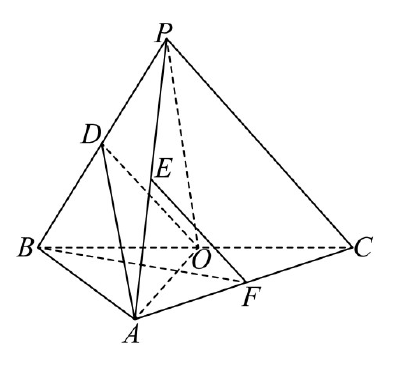
\includegraphics[width=\linewidth]{figures/2023_yi_wen_q19.png}
\end{minipage}
\vspace{-3em}
\item（12分）

已知函数$f(x)=\left(\dfrac1x+a\right)\ln(1+x)$. 

\subq{（1）}{当$a=-1$时，求曲线$y=f(x)$在点$(1,f(1))$处的切线方程；}

\subq{（2）}{若函数$f(x)$在$(0,+\infty)$单调递增，求$a$的取值范围.}

\item（12分）

已知椭圆$C:\dfrac{y^2}{a^2}+\dfrac{x^2}{b^2}=1(a>b>0)$的离心率是$\dfrac{\sqrt5}{3}$，点$A(-2,0)$在$C$上. 

\subq{（1）}{求$C$方程；}

\subq{（2）}{过点$(-2,3)$的直线交$C$于$P,Q$两点，直线$AP,AQ$与$y$轴的交点分别为$M,N$，证明：线段$MN$的中点为定点.}
\end{examanswers}

\examsection{四、选做题：共10分. 请考生在第22、23题中任选一题作答. }
\begin{examanswers}[start=22]
\item（10分）【选修4-4：坐标系与参数方程】

在直角坐标系$xOy$中，以坐标原点$O$为极点，$x$轴正半轴为极轴建立极坐标系，曲线$C_1$的极坐标方程为$\rho=2\sin\theta\left(\dfrac\pi4\leq\theta\leq\dfrac\pi2\right)$，曲线$C_2:$\linsys{x=2\cos\alpha,\\y=2\sin\alpha}（$\alpha$为参数，$\dfrac\pi2<\alpha<\pi$）. 

\subq{（1）}{写出$C_1$的直角坐标方程；}

\subq{（2）}{若直线$y=x+m$既与$C_1$没有公共点，也与$C_2$没有公共点，求$m$的取值范围.}

\item（10分）【选修4-5：不等式选讲】

已知$f(x)=2|x|+|x-2|$. 

\subq{（1）}{求不等式$f(x)\leq6-x$的解集；}

\subq{（2）}{在直角坐标系$xOy$中，求不等式组\linsys{f(x)\leq y,\\x+y-6\leq0}所确定的平面区域的面积.}
\end{examanswers}

\end{document}
